\documentclass[9pt,twocolumn,twoside]{../../styles/osajnl}
\usepackage{fancyvrb}
\journal{i524} 

\title{An overview of the open source log management tool - Graylog}

\ociscodes{Cloud, I524}
\author[1]{Rahul Singh}

\affil[1]{School of Informatics and Computing, Bloomington, IN 47408, U.S.A.}

\affil[*]{Corresponding authors: rahpsing@iu.edu}

\dates{\today}

\ociscodes{Cloud, I524}

% replace this with your url in github/gitlab
\doi{\url{https://github.com/cloudmesh/sp17-i524/blob/master/paper2/S17-IR-2036/report.pdf}}


\begin{abstract}
Graylog is an open source log management tool
that allows an organization to collect, organize and analyze large
amounts of data from its network activity. It enhances the basic log
management functionality by providing network traffic analysis, lucene
syntax based search, drill-down analysis of data using field
statistics and generates trigger actions based alert notifications. It
integrates with other open source technologies to address a larger
distributed system.
\newline
\end{abstract}

\setboolean{displaycopyright}{true}

\begin{document}

\maketitle

\section{Introduction}
\emph{Graylog} \cite{www-graylog-org} allows management of an
organization's computing resources in a consistent way. It allows us
to centrally collect and manage log messages of an organization’s
complete infrastructure. A user can perform search on terabytes of log
data to discover number of failed logins, find application errors
across all servers or monitor the activity of a suspicious user
id. Graylog works on top of \emph{ElasticSearch}
\cite{www-elasticsearch-wiki} and \emph{MongoDB}
\cite{www-mongodb-wiki} to facilitate this high availability
searching. It provides a \emph{Lucene} \cite{www-apachelucene-org}
like query language, a processing pipeline for data transformation,
alerting abilities and much more. Graylog enables organizations, at a
fraction of the cost, to improve IT operations efficiency, security,
and reduce the cost of IT \cite{www-graylog-hightech}.


\section{Architecture}

Graylog is written in Java and uses a few key open source technologies
like ElasticSearch and MongoDB. Additionally, for a larger setup
\emph{Apache Kafka} \cite{www-apachekafka-org} or \emph{RabbitMQ}
\cite{www-rabbitmq-com} could be integrated to implement queueing. A
basic Graylog cluster consists of the following components:
\newline
\newline
Graylog server - It is the actual log processor system also
responsible for implementing security. The Graylog server nodes shall
be operated on the fastest CPU's available.
\newline
\newline
Graylog web UI - It is the Graylog web user interface where one can
view histograms, dashboards and create alerts.
\newline
\newline
MongoDB - MongoDB stores Graylog configuration information and the non
queried log messages. It's prime purpose in the architecture is Metadata
Management \cite{www-graylogprocessing-severalnines}.
\newline
\newline
ElasticSearch - ElasticSearch is useful for storing actual log data
and perform search operations on them. ElasticSearch nodes should have
as much RAM as possible and the fastest disks linked to them. Messages
are only stored on ElasticSearch nodes. If we have data loss on
ElasticSearch, all messages are gone – except if the administrator has
created backups of the indices.

\begin{figure}[htbp]
\centering
\fbox{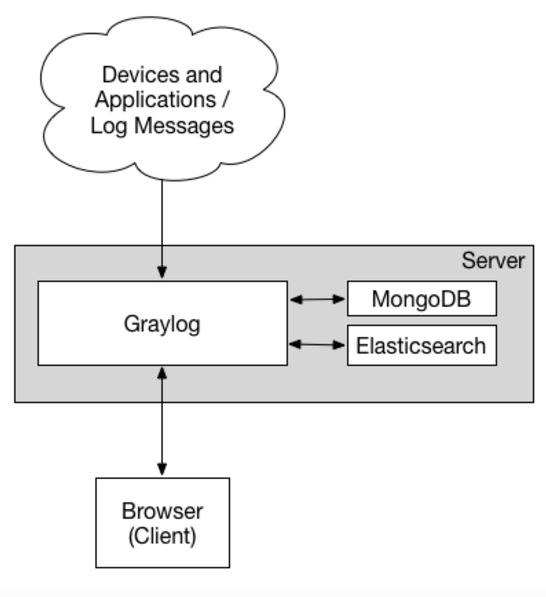
\includegraphics[width=40mm,height=40mm]{images/min_architecture_graylog}}
\caption{Graylog minimum architecture \cite{www-graylog-docs}}
\label{fig:Graylog Minimum Architecture}
\end{figure}

\section{Graylog Use Cases}

\subsection{Computer And Network Security}

The best way for intrusion detection is to monitor activity of all the
devices in the network. Graylog allows a user to keep track of all
failed logins, rejected network connections or exceptions in the flow
of the application. It also allows a user to integrate other
\emph{Intrusion Detection Systems (IDS)} \cite{www-ids-wiki} to
correlate detected activity with logs from all across the
infrastructure \cite{www-graylog-org}.

\subsection{Centralized IT management}

Logging into every system and parsing the plain text log files to find
meaningful data is an arduous task for any IT engineer. Graylog allows
us to centrally collect all syslog and eventlog messages of the
complete infrastructure thus allowing to solve production issues in
real time. It does so by allowing the administrator to setup alerts
for any trigger actions like performance degradation or exceptions.

\subsection{Development and DevOps}

Graylog allows on demand monitoring of distributed applications by
giving tiered access to any developer in the organization to view
system and application logs. It works on top of elastic search nodes
to facilitate search operation on terabytes of log data in a matter
of milliseconds. In case of a customer operation resulting in an
error, a developer shall need to search the logs with the customer id
and locate the relevant logs to find the root cause of the problem.

\section{Graylog Modules}


\subsection{Sending in log data}

Graylog needs a log source to serve its purpose. The message input
section is launched from the System - Inputs section from the web
interface (or the \emph{REST API} \cite{www-rest-wiki}) and can be
configured without the need to restart any part of the system
\cite{www-graylog-sending_data}.

Graylog is able to accept and parse \emph{RFC 5424}
\cite{www-rfc5424-ietf} and \emph{RFC 3164} \cite{www-rfc3164-ietf}
compliant syslog messages and the Graylog Extended Log Format (GELF)
\cite{www-graylog-sending_data}. For any devices on the network that
do not publish RFC compliant syslog messages we need to make use of
the plaintext messages.  The GELF is a log format that avoids the
shortcomings of classic plain syslog by providing optional
compression, fixed structure and limits payload length to 1024
bytes. Syslog is preferred for direct logging by machines in the
network while GELF is suitable for logging from within the
applications.

\subsection{Search}

As Graylog uses ElasticSearch to facilitate searching, the search
syntax followed is very close to the Lucene syntax which is the
underlying implementation of Elastic Search. By default, search is
performed over all fields unless a specific field is specified in the
search query. Search features like fuzzy, wildcard, range searches
provided by Elastic Search API can be used to gain deeper insight to
data. Graylog also provides a time frame selector which defines the
time range over which the search shall be performed. The time selector
could be relative, absolute or keyword based.
Graylog also allows a user to save his searches to view it later. A
user needs to save his search by a unique name and could load it later
from the system, under the saved search selector.
 
Graylog automatically constructs a histogram for the search
results. The histogram depicts the concise number of messages received
grouped by a certain time period that is adjustable.  Based on a user’s
recent search query, graylog also allows you to distinguish data that
are not searched upon very often and thus can be archived on cost
effective storage drives.

\subsection{Log Streams}

Graylog allows a user to create a set of rules to route messages into
user defined categories. A user could create a stream called 'Database
errors' and create a rule to direct all messages with the source
attribute as 'database' to that stream. Thus, the stream 'Database
errors' shall catch every error message from the system's database
hosts. A message shall be routed into every stream that has the
corresponding matching rule for the message. A message thus, can be
part of many streams and not just one \cite{www-graylog-streams}.

\subsection{Alerts}

Graylog alerts are periodical searches that can trigger some
notifications when a defined condition is satisfied
\cite{www-graylog-alerts}. To get notified when more than 50
exceptions occur in the range of a minute, an alert can be created
with the desired conditions.  While defining alerts, a user can also
specify the method of notification once the alert condition is
met. Notifications can be obtained by an email or by an HTTP request
to an endpoint in the system.

\subsection{Dashboards}

Graylog provides visualization through creation of dashboards that
allows a user to build pre-defined views on his data to assemble all
of his important data only a single click away
\cite{www-graylog-dashboards}. Any search result or metric shall be
added as a widget on the dashboard to observe trends in one single
location.  A user can also add search result metrics like result
count, statistical values, field value charts and stack charts to the
dashboard. These dashboards can also be shared with other users in the
organization.

\subsection{Graylog REST API}

Both configuration settings and log data are available through the
Graylog REST API.  The Graylog web interface uses Graylog Rest API
internally to interact with the Graylog cluster. Graylog REST API
could be used for automation or integrating Graylog into another
system, such as monitoring or ticket systems
\cite{www-graylog-restapi}. Thus a network administrator can easily
integrate Graylog into his evolving architecture and build reports and
analysis.

\subsection{Filtering messages}

Graylog can use \emph{Drools} \cite{www-drools-org} to evaluate all
incoming messages against a user defined rules file. To discard any
message before its written to elastic search or to forward it to
another system, one can use Drools rules to perform custom filtering
\cite{www-graylog-blacklisting}.

\section{Comparision with Splunk}
\emph{Splunk} \cite{www-splunk} is considered as one of the best log
management tools available and is Graylog's biggest competitor. Splunk
started as a log analysis tool but has now grown into a full machine
generated data processing platform. Splunk works on almost every
format of log data unlike graylog, but has a higher setup cost. To
deploy Splunk in a high scale environment, a user needs to install and
configure a dedicated cluster. Table below represents a comparision of
Graylog and Splunk for a few basic factors.

\begin{table}[htbp]
\centering
\caption{\bf Comparision of Graylog and Splunk}\cite{www-logmanagementtools-blog} \cite{www-graylogvssplunk-article}
\begin{tabular}{ccc}
\hline
Parameter & Graylog & Splunk \\
\hline
Business Model& Opensource & Commercial software \\
Setup Time & Needs time & No time\\
Learning Curve & Difficult & Simple\\
Filetypes & syslog,gelf & Many\\
Security & Good & Good\\
Apps Supported & Low & Very high\\
\hline
\end{tabular}
  \label{tab:shape-functions}
\end{table}


\section{Conclusion}
Graylog makes big data analytics affordable by providing an open
source solution that allows organizations to realize the benefits of
collecting and analyzing log data and thus improving operational
efficiency at a reduced cost of IT. It provides an effective set of
features to be adapted by any small to medium size organization. Alert
notifications, sharing of dashboards and message filtering provide
most features that any network administrator desires from a log
management system. Being an open source tool it is cost effective
compared to other log systems. Graylog provides centralized monitoring
and management of large scale distributed systems from a single point
of control. However, it needs an environment to be setup before it can
be operational. It has a steep learning curve with the responsibility
of managing the MongoDB and ElasticSearch instances being completely
managed by the user. Hence, the choice to choose Graylog as an
organization's log management tool directly relies on the resources in
terms of either time or money that it chooses to employ.


% Bibliography

\bibliography{references}

 
\section*{Author Biographies}
\begingroup
\setlength\intextsep{0pt}
\begin{minipage}[t][3.2cm][t]{1.0\columnwidth} % Adjust height [3.2cm]
                                               % as required for
                                               % separation of bio
                                               % photos.
  \begin{wrapfigure}{L}{0.25\columnwidth}
    
\includegraphics[width=0.25\columnwidth]{images/rahul_singh.jpg}
  \end{wrapfigure}
  \noindent
{\bfseries Rahul Singh} received his B.E. (Computer Engineering) from
University of Mumbai, India. He is currently pursuing his Masters in
Computer Science at Indiana University Bloomington.

\end{minipage}
\endgroup

\end{document}
